Pierwszym krokiem algorytmu wykrywania logo \bk, jest przetwarzanie wstępne. Celem przetwarzania wstępnego jest zmniejszenie rzeczywistego rozmiaru obrazu, względna poprawa jego jakości oraz usunięcie zakłóceń.

\subsection{Skalowanie obrazu}
\todo{pozmieniać te obrazki bo dalej nic z nich nie wynika}
Celem skalowania obrazu jest stworzenie nowego obrazu o~zmienionym rozmiarze, wykorzystując do tego obraz oryginalny. W~przypadku projektowanego systemu, obraz analizowany jest poddawany skalowaniu aby zmniejszyć jego rzeczywisty rozmiar, celem uproszczenia dalszych obliczeń.

Do zmiany rozdzielczości obrazu cyfrowego zwykle wykorzystuje się metody interpolacji. Algorytmy tego typu można podzielić na algorytmy nieadaptacyjne oraz adaptacyjne. Pierwsza grupa dokonuje interpolacji w~ustalony z~góry sposób, niezależnie od zawartości przetwarzanego obrazu. Algorytmy adaptacyjne zmieniają sposób przetwarzania pikseli, biorąc pod uwagę cechy aktualnie przetwarzanego fragmentu. Adaptacja pozwala na zwiększenie jakości wizualnej, zwiększając przy tym koszt obliczeniowy~\cite{swierczynski2008podwyzszanie}.

W~ramach projektu przeanalizowałem działanie trzech algorytmów nieadaptacyjnych: 
\begin{itemize}
    \item interpolacja najbliższym sąsiadem,
    \item interpolacja dwuliniowa,
    \item interpolacja dwukubiczna.
\end{itemize}

Wymienione algorytmy różnią się ilością punktów branych pod uwagę podczas obliczania jasności piksela w~obrazie wynikowym. W~pierwszym kroku każdego algorytmu oblicza się w~którym miejscu w~obrazie wejściowym znajduje się rozpatrywany punkt obrazu wyjściowego. Dokonuje się tego poprzez obliczenie współczynników skalowania, zgodnie z~wzorami~\ref{eqn:wsp-skalowania-x}~i~\ref{eqn:wsp-skalowania-y}.

\begin{equation}
    \label{eqn:wsp-skalowania-x}
    r_{x} = \frac{\mathrm{width}_{input}}{\mathrm{width}_{output}}
\end{equation}

\begin{equation}
    \label{eqn:wsp-skalowania-y}
    r_{y} = \frac{\mathrm{height}_{input}}{\mathrm{height}_{output}}
\end{equation}

Na podstawie współczynników $r_{x}, r_{y}$ dla piksela $(i, j)$ obrazu wyjściowego oblicza się pozycję~$(x, y)$ w~obrazie wejściowym, wykorzystując zależność \ref{eqn:skalowanie}.

\begin{equation}
    \label{eqn:skalowanie}
    \begin{array}{ll}
        x = i \cdot r_{x} & y = j \cdot r_{y}
    \end{array} 
\end{equation}

\subsubsection{Interpolacja najbliższym sąsiadem}
Interpolacja metodą najbliższego sąsiada jest najprostszą metodą zmiany rozmiaru obrazu cyfrowego. Jest to metoda wymagająca najmniejszej mocy obliczeniowej i~jest jedyną metodą nie powodującą rozmycia obrazu wynikowego. W~przetwarzaniu obrazów jest najczęściej wykorzystywana do zmiany rozmiaru zdjęć zawierających kody kreskowe lub zrzutów ekranu aplikacji okienkowych.

Algorytm interpolacji najbliższym sąsiadem działa w~następujący sposób. Dla każdej obliczonej pary $(x,y)$ odpowiadającej pikselowi $(i, j)$ w~obrazie wyjściowym, wybierany jest rzeczywisty piksel $(\hat{x}, \hat{y})$ obrazu wejściowego, którego odległość punktu docelowego jest najmniejsza (czyli jest najbliższym sąsiadem obliczonego piksela).

\todo{wstawić jakiś obrazek na temat tego algorytmu}

W~stworzonym rozwiązaniu, algorytm interpolacji dwuliniowej jest implementowany przez  obiekty klasy \texttt{POBR::NearestNeighbourInterpolationResizer}. Wyniki działania tego algorytmu zostały przedstawione na rysunku~\ref{fig:nearestneighbour-result}. 

\begin{figure}[h]
    \centering
    \subfloat[100x100px]{{\includegraphics[scale=1.65]{figures/100x100/nn.pdf}}}
    \qquad
    \subfloat[200x200px]{{\includegraphics[scale=0.32]{./figures/200x200.jpg} }}%
    \qquad
    \subfloat[400x400px]{{\includegraphics[scale=0.405]{./figures/400x400/nn.pdf} }}%
    \caption{Efekt działania algorytmu interpolacji najbliższym sąsiadem na przykładzie zmniejszania logo \bk z~rozmiaru 200x200px do 100x100px oraz zwiększania do rozmiaru 400x400px}
    \label{fig:nearestneighbour-result}
\end{figure}

Obrazy przetworzone za pomocą algorytmu interpolacją najbliższego sąsiada cechują się blokowatością. Brak rozmycia powoduje że obraz traci naturalny wygląd. Jest to jednak metoda najszybsza, warta rozważenia w~zadanich automatycznego wykrywania obiektów.

\subsubsection{Interpolacja dwuliniowa}
Algorytm interpolacji dwuliniowej jest algorytmem nieadaptacyjnym, nieco bardziej zaawansowanym niż pokrewny algorytm najbliższego sąsiada. Wartość każdego piksela obrazu wynikowego jest obliczana na podstawie czterech sąsiednich punktów obrazu wejściowego~\cite{algorytmy:bilinear}.

Na podstawie informacji o~docelowym punkcie, wybiera się cztery najbliższe punkty $F_{0,0}, F_{0,1}, F_{1,0}, F_{1,1}$, tak jak to przedstawiono na~\ref{fig:bilinear-result} (żółtym kolorem zaznaczono punkt obliczony z~wzorów~\ref{eqn:skalowanie}). 

\begin{figure}[h]
    \centering
    \includegraphics[width=0.6\columnwidth]{figures/bi2.png}
    \caption{Dobór sąsiednich punktów w~algorytmie interpolacji dwuliniowej~\cite{algorytmy:bilinear}}
    \label{fig:bilinear-example}
\end{figure}

Następnie trzykrotnie przeprowadza się interpolację pomiędzy punktami, najpierw dwa razy w~kierunku poziomym pomiędzy $F_{0,0}$~i~$F_{1,0}$ oraz $F_{0,1}$~i~$F_{1,1}$ i~ostatni raz pomiędzy wynikami poprzednich interpolacji, zgodnie ze wzorem~\ref{eqn:interpolacja}. Proces ten należy powtórzyć dla każdej składowej koloru z~osobna~\cite{algorytmy:bilinear}.

\begin{equation}
    \label{eqn:interpolacja}
    \begin{array}{l}
        F_{a,0} = (1-a) \cdot F_{0,0} + a \cdot F_{1,0} \\
        F_{a,1} = (1-a) \cdot F_{0,1} + a \cdot F_{1,1} \\
        F_{a,b} = (1-b) \cdot F_{a,0} + b \cdot F_{0,1} \\
    \end{array} 
\end{equation}

W~stworzonym rozwiązaniu, algorytm interpolacji dwuliniowej jest implementowany przez  obiekty klasy \texttt{POBR::BilinearInterpolationResizer}. Wyniki działania tego algorytmu zostały przedstawione na rysunku~\ref{fig:bilinear-result}.

\begin{figure}[h]
    \centering
    \subfloat[100x100px]{{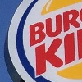
\includegraphics[scale=1.61]{figures/100x100/bl.pdf}}}
    \qquad
    \subfloat[200x200px]{{\includegraphics[scale=0.32]{./figures/200x200.jpg} }}%
    \qquad
    \subfloat[400x400px]{{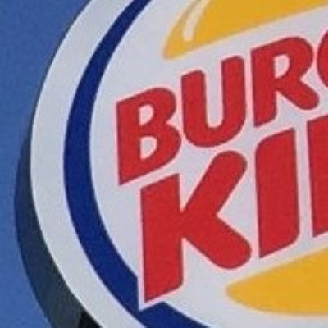
\includegraphics[scale=0.405]{./figures/400x400/bl.pdf} }}%
    \caption{Efekt działania algorytmu interpolacji dwuliniowej na przykładzie zmniejszania logo \bk z~rozmiaru 200x200px do 100x100px oraz zwiększania do rozmiaru 400x400px}
    \label{fig:bilinear-result}
\end{figure}

Algorytm interpolacji dwuliniowej jest zdecydowanie bardziej skomplikowanym algorytmem przetwarzania. W~wyniku jego działania, obraz wyjściowy jest rozmyty, co jednak pozwala na zachowanie naturalnego wyglądu obrazu. Mimo brania pod uwagę czterech pikseli, metoda ta niewiele mocniej obciąża procesor. 

\subsubsection{Interpolacja dwukubiczna}
\todo{Opisać algorytm interpolacji dwukubicznej, wstawić wyniki interpolacji, opisać działanie.}

\todo{zasada działania algorytmu}

\todo{prezentacja działania algorytmu - opis, zdjecie, komentarz}

\todo{wady i zalety algorytmu}
\begin{figure}[h]
    \centering
    \subfloat[100x100px]{{\includegraphics[scale=1.61]{figures/100x100/bc.pdf}}}
    \qquad
    \subfloat[200x200px]{{\includegraphics[scale=0.32]{./figures/200x200.jpg} }}%
    \qquad
    \subfloat[400x400px]{{\includegraphics[scale=0.405]{./figures/400x400/bc.pdf} }}%
    \caption{Efekt działania algorytmu interpolacji dwukubicznej na przykładzie zmniejszania logo \bk z~rozmiaru 200x200px do 100x100px oraz zwiększania do rozmiaru 400x400px}
    \label{fig:bicubic-result}
\end{figure}

\subsection{Filtracja zakłóceń}
\todo{Opisać algorytm filtracji zakłóceń - filtracja medianowa. Znaleźć źródła.}